\pagestyle{quadrado}
\label{quadrado}

\begin{textblock*}{5.625in}(0pt,0pt)%
\vspace*{-1.45cm}
\hspace*{-1.8cm}\includegraphics*[width=112mm]{./imgs/QUADRADO.png}
\end{textblock*}

\pagebreak

\hspace{.5cm}

\begin{center}
\hspace*{-1cm}\raisebox{5.5cm}{\rotatebox[origin=t]{90}{\Formular{\textbf{Lançamento}}}}
\hspace*{1cm}
\includegraphics[width=70mm]{./grid/zuker.jpeg}
\end{center}

\hspace*{-7cm}\hrulefill\hspace*{-7cm}

%\hspace*{-2cm}\_\_\_\_\_\_\_\_\_\_\_\_\_\_\_\_\_\_\_\_\_\_\_\_\_\_\_\_\_\_\_\_\_\_\_\_\_\_\_\_\_\_\_\_\_\_\_\_\_\_\_\_\_\_\_\_\_\_\_\_\_\_\_\_\_\_\_\_\_\_\_\_\_\_

\medskip

\noindent{}O medo, em sua faceta promíscua com mecanismo de governar neoliberal, é o fio condutor que percorre os quatro ensaios de {\slsc{Em rota de fuga}}. Marcado por um olhar plurívoco, que perpassa a história da arte, Sade, o cinema, as vozes amazônicas e as práticas de escrita contemporâneas, o ensaísta perscruta os desdobramentos dessa política para pensar outros mundos e outras formas de sensibilidade que criem efetivas rotas de fuga do círculo de violência neoliberal.

\vfill

\hspace*{-.4cm}\begin{minipage}[c]{1\linewidth}
\small{
{\Formular{\textbf{
\hspace*{-.1cm}Título: Em rota de fuga\\
Autor: Fábio Zuker\\ 
Editora: quadradocirculo\\
Páginas: 181\\
Formato: 11x18cm\\
Preço: R\$ 49,90\\
ISBN: 978-85-7715-621-4
}}}}
\end{minipage}


\pagebreak

\hspace{.5cm}

\begin{center}
\hspace*{-.5cm}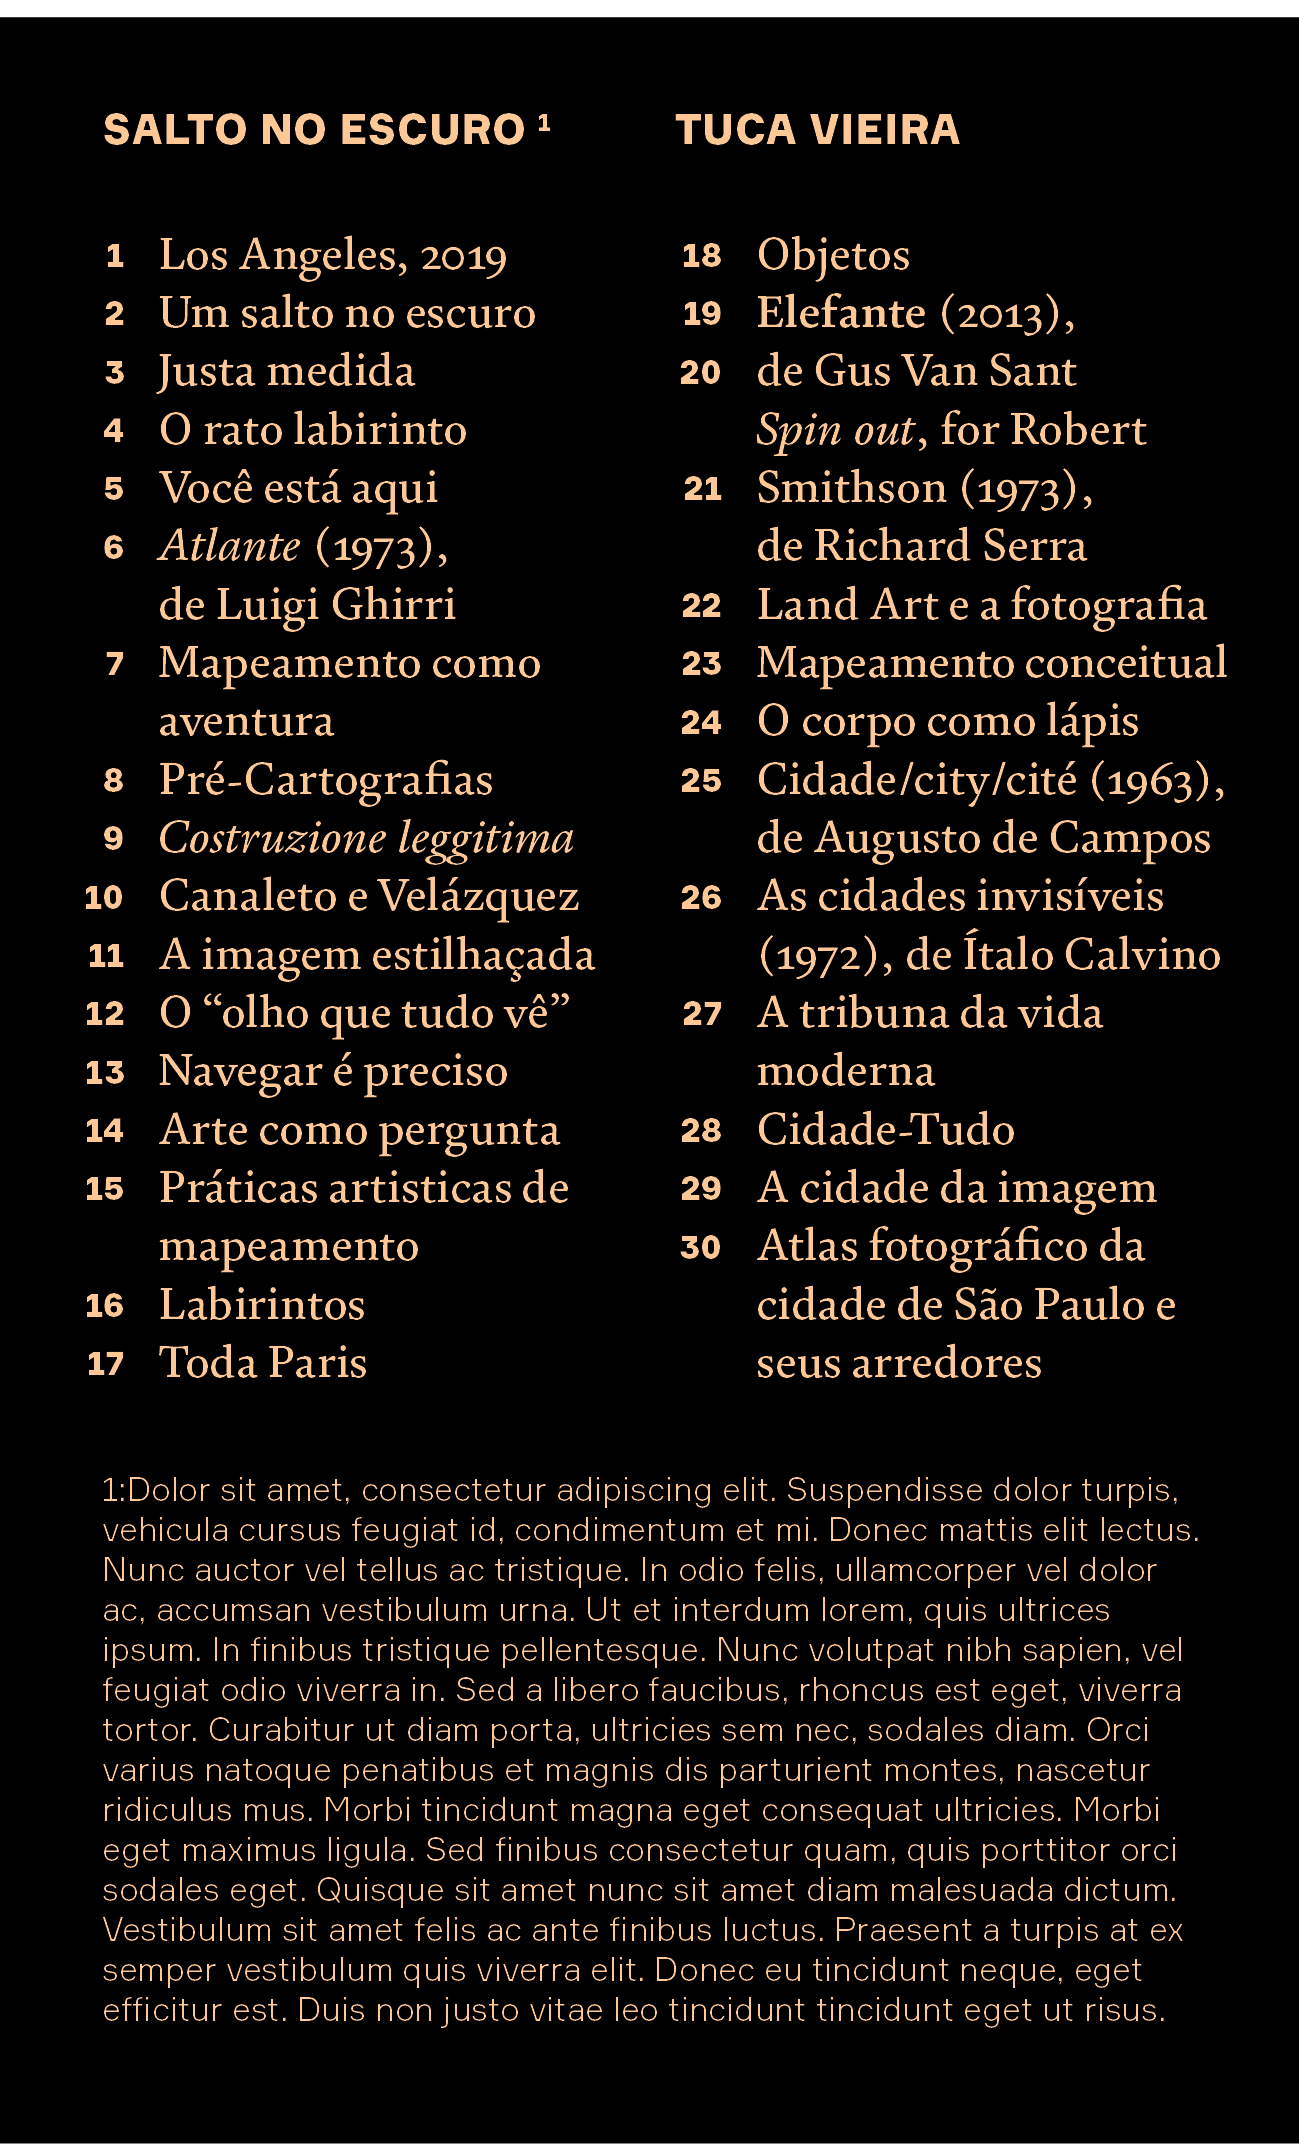
\includegraphics[width=42.4mm]{./imgs/escuro.png}
\end{center}

\hspace*{-7cm}\hrulefill\hspace*{-7cm}

%\hspace*{-2cm}\_\_\_\_\_\_\_\_\_\_\_\_\_\_\_\_\_\_\_\_\_\_\_\_\_\_\_\_\_\_\_\_\_\_\_\_\_\_\_\_\_\_\_\_\_\_\_\_\_\_\_\_\_\_\_\_\_\_\_\_\_\_\_\_\_\_\_\_\_\_\_\_\_\_


\medskip

\noindent{}Em {\slsc{Salto no escuro}}, o renomado fotógrafo Tuca Vieira percorre diversos centros urbanos, labirintos e criações artísticas para pensar o que é a cidade e o espaço geográfico contemporâneos. Marcado pela multiplicidade de caminhos, o autor instiga a novas possiblidades e percepções diante da aceleração da vida e da nova realidade impostas pela tecnologia. Como escreve, trata"-se de observar o abismo com o qual nos defrontamos, antes de saltar no escuro desses espaços mecânicos e artificiais.

\vfill

\hspace*{-.4cm}\begin{minipage}[c]{1\linewidth}
\small{
{\Formular{\textbf{
\hspace*{-.1cm}Título: Salto no escuro\\
Autor: Tuca Vieira\\ 
Editora: quadradocirculo\\
Páginas: 490\\
Formato: 11x18cm\\
Preço: R\$ 79,90\\
ISBN: 978-85-7715-622-1
}}}}
\end{minipage}

\pagebreak